\begin{figure}[t]
\centering
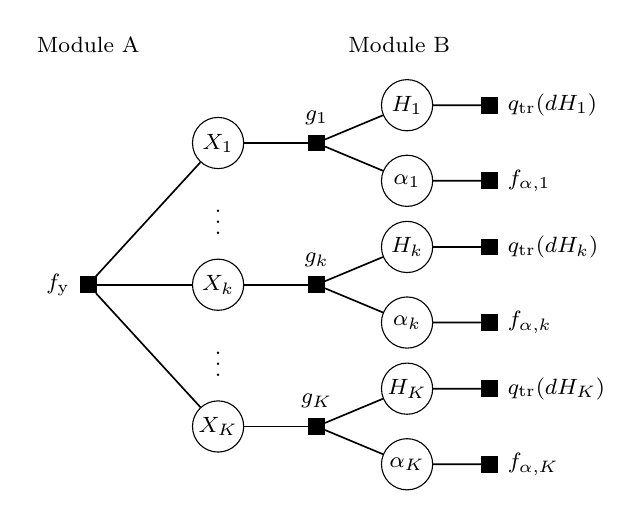
\begin{tikzpicture}[
 font=\footnotesize,
 fgvariable/.style={circle,draw,minimum size=6.5mm,inner sep=1pt},
 fgfactor/.style={rectangle,draw,fill=black,minimum size=2mm,inner sep=0pt},
 fgedge/.style={semithick}]
 \node[fgfactor,label=left:{$f_{\rm y}$}] (fy) at (0,0) {};
 \node[align=center] at (0,3.05) {Module A};
 \node[align=center] at (3.95,3.05) {Module B};
 \foreach \idx/\row in {1/1.8,k/0,K/-1.8} {
   \node[fgvariable] (x\idx) at (1.65,\row) {$X_{\idx}$};
   \node[fgfactor,label=above:{$g_{\idx}$}] (g\idx) at (2.9,\row) {};
   \node[fgvariable] (h\idx) at (4.05,{\row+0.48}) {$H_{\idx}$};
   \node[fgvariable] (a\idx) at (4.05,{\row-0.48}) {$\alpha_{\idx}$};
   \node[fgfactor,label=right:{$q_{\rm tr}(dH_{\idx})$}]
       (ph\idx) at (5.1,{\row+0.48}) {};
   \node[fgfactor,label=right:{$f_{\alpha,\idx}$}]
       (pa\idx) at (5.1,{\row-0.48}) {};
   \draw[fgedge] (fy) -- (x\idx);
   \draw[fgedge] (x\idx) -- (g\idx);
   \draw[fgedge] (g\idx) -- (h\idx) -- (ph\idx);
   \draw[fgedge] (g\idx) -- (a\idx) -- (pa\idx);
 }
 \node at (1.65,0.9) {$\vdots$};
 \node at (1.65,-0.9) {$\vdots$};
\end{tikzpicture}
\caption{Factor graph of \eqref{eq:working-posterior}, with the
observation factors grouped into $f_{\rm y}$. Circles denote variable
nodes and filled squares denote factor nodes. Each $X_k$ or $H_k$
node contains $D$ complex coefficients. The likelihood couples the
user blocks, while $g_k$ imposes $X_k=\alpha_kH_k$.}
\label{fig:twc-factor-graph}
\end{figure}
